\clearpage
\subsubsection{SPIDER}

% add image spider3.png
\begin{figure}[htb]
    \centering
    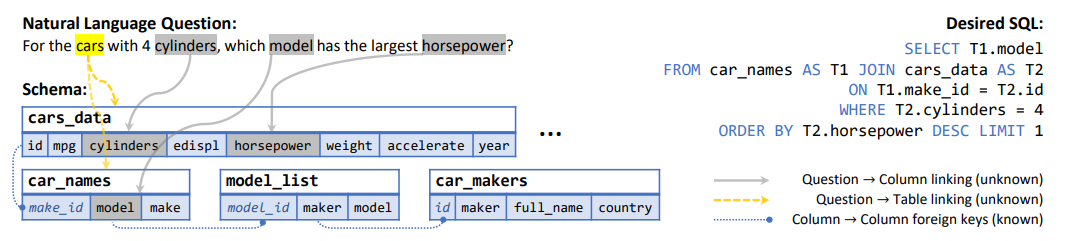
\includegraphics[width=0.9\textwidth]{pics/db/Spider3.png}
    \caption{A difficult text-to-SQL task from the Spider dataset.\cite{wang_rat-sql_2021}}
    \label{fig:Spider3}
\end{figure}

The SPIDER database contains 10K questions and 5K+ complex SQL queries covering 138 different domains across 200 databases. As opposed to previous datasets (most of which used only one database), this one incorporates multiple datasets. Creating this dataset took 11 Yale University students, 1,000 man-hours in total.

Spider contains queries with a lot of intricate SQL elements. In comparison to the sum of the previous Text-to-SQL datasets, Spider comprises around twice as many nested queries and ten times as many ORDER BY (LIMIT) and GROUP BY (HAVING) components.

Creating this corpus was primarily motivated by the desire to tackle complex queries and generalize across databases without requiring multiple interactions.

\begin{figure}[htb]
    \centering
    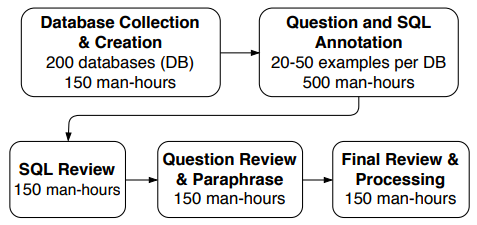
\includegraphics[width=0.6\textwidth]{pics/db/Spider.png}
    \caption{Process of creating SPIDER dataset\cite{yu_spider_2019}}
    \label{fig:Spider}
\end{figure}

Creating a dataset involves three main aspects: SQL pattern coverage, SQL consistency, and question clarity. Several databases from WikiSQL are included in the dataset. The table is complex as it links several tables with foreign keys. In SPIDER, SQL queries include: SELECT with multiple columns and aggregations, WHERE, GROUP BY, HAVING, ORDER BY, LIMIT, JOIN, INTERSECT, EXCEPT, UNION, NOT IN, OR, AND, EXISTS, LIKE.

The complexity of the dataset increases and the accuracy of solutions drops as the number of foreign keys in the database increases. This is mainly due to the difficulty in selecting the relevant column and table names from a complex database schema. Furthermore, complex database schemas present a major challenge for the model to accurately capture the relationship between different tables which involve foreign keys. SQL queries with a higher number of foreign keys tend to join more tables, suggesting a need for more effective methods to encode the connection between tables with foreign keys.

\subsubsection*{SQL Hardness Criteria}

In order to gain a better understanding of how the model performs on different queries, we have divided SQL queries into four difficulty levels: easy, medium, hard, and extra hard. This classification is based on the number of SQL components, selections, and conditions. Queries that contain multiple SQL keywords (e.g., GROUP BY, ORDER BY, INTERSECT, nested subqueries, column selections, aggregators) are generally considered more complex. For example, a query is considered hard if it includes more than two SELECT columns, more than two WHERE conditions, and GROUP BY two columns, or contains EXCEPT or nested queries. If it contains even more additions on top of that, it is considered extra hard.

\begin{figure}[htb]
    \centering
    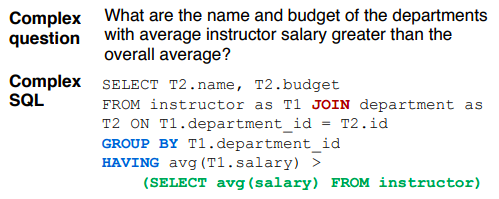
\includegraphics[width=0.8\textwidth]{pics/db/Spider2.png}
    \caption{Example of Question-Query set from SPIDER\cite{yu_spider_2019}}
    \label{fig:Spider2}
\end{figure}


SPIDER's exact matching accuracy\ref{eval} was 12.4\% compared to existing state-of-the-art models. As a result of its low accuracy, SPIDER presents a strong research challenge. Current SPIDER accuracy is above 75.5\% with an exact set match without values (refers to values in the WHERE clause) and above 72.6\% with values using PICARD\ref{picard}.

The SPIDER challenge is a research competition dedicated to developing cutting-edge Text-to-SQL and Semantic Parsing solutions. In this challenge, participants strive to develop algorithms that can automatically generate structured SQL queries from natural language input, to improve the performance and accuracy of Text-to-SQL models.

In this challenge, numerous state-of-the-art Text-to-SQL solutions have been proposed, such as the Spider model. This model uses a combination of recurrent and convolutional neural networks to learn the mapping between natural language and SQL queries. This model also has a hierarchical structure, which allows it to process the natural language input more effectively, thereby allowing it to handle complex queries and variations in language with greater precision and accuracy. This model successfully generates accurate and efficient SQL queries from natural language inputs.

One difference between the SPIDER and WikiSQL challenges is the specific dataset that is used for evaluation. The SPIDER challenge uses a dataset of complex SQL queries and natural language questions derived from real-world databases, while the WikiSQL challenge uses a dataset of more straightforward SQL queries and natural language questions derived from Wikipedia articles. This difference in the dataset can affect the performance and accuracy of the models on the different tasks.

Another difference is in the evaluation metrics used. The SPIDER challenge evaluates the models using execution accuracy and natural language understanding metrics, while the WikiSQL challenge evaluates the models using only execution accuracy. This difference in the evaluation metrics can affect how the models are trained and their performance on the tasks. We will discuss the evaluation metrics used in the SPIDER challenge in more detail in the next section\ref{eval}.